% Options for packages loaded elsewhere
\PassOptionsToPackage{unicode}{hyperref}
\PassOptionsToPackage{hyphens}{url}
%
\documentclass[
  ignorenonframetext,
]{beamer}
\usepackage{pgfpages}
\setbeamertemplate{caption}[numbered]
\setbeamertemplate{caption label separator}{: }
\setbeamercolor{caption name}{fg=normal text.fg}
\beamertemplatenavigationsymbolsempty
% Prevent slide breaks in the middle of a paragraph
\widowpenalties 1 10000
\raggedbottom
\setbeamertemplate{part page}{
  \centering
  \begin{beamercolorbox}[sep=16pt,center]{part title}
    \usebeamerfont{part title}\insertpart\par
  \end{beamercolorbox}
}
\setbeamertemplate{section page}{
  \centering
  \begin{beamercolorbox}[sep=12pt,center]{part title}
    \usebeamerfont{section title}\insertsection\par
  \end{beamercolorbox}
}
\setbeamertemplate{subsection page}{
  \centering
  \begin{beamercolorbox}[sep=8pt,center]{part title}
    \usebeamerfont{subsection title}\insertsubsection\par
  \end{beamercolorbox}
}
\AtBeginPart{
  \frame{\partpage}
}
\AtBeginSection{
  \ifbibliography
  \else
    \frame{\sectionpage}
  \fi
}
\AtBeginSubsection{
  \frame{\subsectionpage}
}
\usepackage{amsmath,amssymb}
\usepackage{lmodern}
\usepackage{ifxetex,ifluatex}
\ifnum 0\ifxetex 1\fi\ifluatex 1\fi=0 % if pdftex
  \usepackage[T1]{fontenc}
  \usepackage[utf8]{inputenc}
  \usepackage{textcomp} % provide euro and other symbols
\else % if luatex or xetex
  \usepackage{unicode-math}
  \defaultfontfeatures{Scale=MatchLowercase}
  \defaultfontfeatures[\rmfamily]{Ligatures=TeX,Scale=1}
  \setmainfont[BoldFont = SF Pro Rounded Semibold]{SF Pro Rounded}
  \setmathfont[]{STIX Two Math}
\fi
\usefonttheme{serif} % use mainfont rather than sansfont for slide text
% Use upquote if available, for straight quotes in verbatim environments
\IfFileExists{upquote.sty}{\usepackage{upquote}}{}
\IfFileExists{microtype.sty}{% use microtype if available
  \usepackage[]{microtype}
  \UseMicrotypeSet[protrusion]{basicmath} % disable protrusion for tt fonts
}{}
\makeatletter
\@ifundefined{KOMAClassName}{% if non-KOMA class
  \IfFileExists{parskip.sty}{%
    \usepackage{parskip}
  }{% else
    \setlength{\parindent}{0pt}
    \setlength{\parskip}{6pt plus 2pt minus 1pt}}
}{% if KOMA class
  \KOMAoptions{parskip=half}}
\makeatother
\usepackage{xcolor}
\IfFileExists{xurl.sty}{\usepackage{xurl}}{} % add URL line breaks if available
\IfFileExists{bookmark.sty}{\usepackage{bookmark}}{\usepackage{hyperref}}
\hypersetup{
  pdftitle={305 Lecture 1.1 - Getting Started},
  pdfauthor={Brian Weatherson},
  hidelinks,
  pdfcreator={LaTeX via pandoc}}
\urlstyle{same} % disable monospaced font for URLs
\newif\ifbibliography
\usepackage{graphicx}
\makeatletter
\def\maxwidth{\ifdim\Gin@nat@width>\linewidth\linewidth\else\Gin@nat@width\fi}
\def\maxheight{\ifdim\Gin@nat@height>\textheight\textheight\else\Gin@nat@height\fi}
\makeatother
% Scale images if necessary, so that they will not overflow the page
% margins by default, and it is still possible to overwrite the defaults
% using explicit options in \includegraphics[width, height, ...]{}
\setkeys{Gin}{width=\maxwidth,height=\maxheight,keepaspectratio}
% Set default figure placement to htbp
\makeatletter
\def\fps@figure{htbp}
\makeatother
\setlength{\emergencystretch}{3em} % prevent overfull lines
\providecommand{\tightlist}{%
  \setlength{\itemsep}{0pt}\setlength{\parskip}{0pt}}
\setcounter{secnumdepth}{-\maxdimen} % remove section numbering
\let\Tiny=\tiny

 \setbeamertemplate{navigation symbols}{} 

% \usetheme{Madrid}
 \usetheme[numbering=none, progressbar=foot]{metropolis}
 \usecolortheme{wolverine}
 \usepackage{color}
 \usepackage{MnSymbol}
% \usepackage{movie15}

\usepackage{amssymb}% http://ctan.org/pkg/amssymb
\usepackage{pifont}% http://ctan.org/pkg/pifont
\newcommand{\cmark}{\ding{51}}%
\newcommand{\xmark}{\ding{55}}%

\DeclareSymbolFont{symbolsC}{U}{txsyc}{m}{n}
\DeclareMathSymbol{\boxright}{\mathrel}{symbolsC}{128}
\DeclareMathAlphabet{\mathpzc}{OT1}{pzc}{m}{it}

\usepackage{tikz-qtree}
% \usepackage{markdown}
%\RequirePackage{bussproofs}
\usetikzlibrary{arrows.meta}
\RequirePackage[tableaux]{prooftrees}
\forestset{line numbering, close with = x}
% Allow for easy commas inside trees
\renewcommand{\,}{\text{, }}


\usepackage{tabulary}

\usepackage{open-logic-config}

\setlength{\parskip}{1ex plus 0.5ex minus 0.2ex}

\AtBeginSection[]
{
\begin{frame}
	\Huge{\color{darkblue} \insertsection}
\end{frame}
}

\renewenvironment*{quote}	
	{\list{}{\rightmargin   \leftmargin} \item } 	
	{\endlist }

\definecolor{darkgreen}{rgb}{0,0.7,0}
\definecolor{darkblue}{rgb}{0,0,0.8}

\newcommand{\starttab}{\begin{center}
\vspace{6pt}
\begin{tabular}}

\newcommand{\stoptab}{\end{tabular}
\vspace{6pt}
\end{center}
\noindent}


\newcommand{\sif}{\rightarrow}
\newcommand{\siff}{\leftrightarrow}
\newcommand{\EF}{\end{frame}}


\newcommand{\TreeStart}[1]{
%\end{frame}
\begin{frame}
\begin{center}
\begin{tikzpicture}[scale=#1]
\tikzset{every tree node/.style={align=center,anchor=north}}
%\Tree
}

\newcommand{\TreeEnd}{
\end{tikzpicture}
%\end{center}
}

\newcommand{\DisplayArg}[2]{
\begin{enumerate}
{#1}
\end{enumerate}
\vspace{-6pt}
\hrulefill

%\hspace{14pt} #2
%{\addtolength{\leftskip}{14pt} #2}
\begin{quote}
{\normalfont #2}
\end{quote}
\vspace{12pt}
}

\newenvironment{ProofTree}[1][1]{
\begin{center}
\begin{tikzpicture}[scale=#1]
\tikzset{every tree node/.style={align=center,anchor=south}}
}
{
\end{tikzpicture}
\end{center}
}

\newcommand{\TreeFrame}[2]{
\begin{columns}[c]
\column{0.5\textwidth}
\begin{center}
\begin{prooftree}{}
#1
\end{prooftree}
\end{center}
\column{0.45\textwidth}
%\begin{markdown}
#2
%\end{markdown}
\end{columns}
}

\newcommand{\ScaledTreeFrame}[3]{
\begin{columns}[c]
\column{0.5\textwidth}
\begin{center}
\scalebox{#1}{
\begin{prooftree}{}
#2
\end{prooftree}
}
\end{center}
\column{0.45\textwidth}
%\begin{markdown}
#3
%\end{markdown}
\end{columns}
}

\usepackage[bb=boondox]{mathalfa}
\DeclareMathAlphabet{\mathbx}{U}{BOONDOX-ds}{m}{n}
\SetMathAlphabet{\mathbx}{bold}{U}{BOONDOX-ds}{b}{n}
\DeclareMathAlphabet{\mathbbx} {U}{BOONDOX-ds}{b}{n}


\newenvironment{oltableau}{\center\tableau{}} %wff format={anchor = base west}}}
       {\endtableau\endcenter}
       
\newcommand{\formula}[1]{$#1$}

\usepackage{tabulary}
\usepackage{booktabs}

\def\begincols{\begin{columns}}
\def\begincol{\begin{column}}
\def\endcol{\end{column}}
\def\endcols{\end{columns}}

\usepackage[italic]{mathastext}
\usepackage{nicefrac}

\definecolor{mygreen}{RGB}{0, 100, 0}
\definecolor{mypink2}{RGB}{219, 48, 122}
\definecolor{dodgerblue}{RGB}{30,144,255}

%\def\True{\textcolor{dodgerblue}{\text{T}}}
%\def\False{\textcolor{red}{\text{F}}}

\def\True{\mathbb{T}}
\def\False{\mathbb{F}}

% This is because arguments didn't have enough space after them
\usepackage{etoolbox}
\AfterEndEnvironment{description}{\vspace{9pt}}
\AfterEndEnvironment{oltableau}{\vspace{9pt}}
\BeforeBeginEnvironment{oltableau}{\vspace{9pt}}
\AfterEndEnvironment{center}{\vspace{12pt}}
\BeforeBeginEnvironment{tabular}{\vspace{9pt}}

\setlength\heavyrulewidth{0pt}
\setlength\lightrulewidth{0pt}

%\def\toprule{}
%\def\bottomrule{}
%\def\midrule{}

\setbeamertemplate{caption}{\raggedright\insertcaption}

\ifluatex
  \usepackage{selnolig}  % disable illegal ligatures
\fi

\title{305 Lecture 1.1 - Getting Started}
\author{Brian Weatherson}
\date{}

\begin{document}
\frame{\titlepage}

\begin{frame}{Aim of Course}
\protect\hypertarget{aim-of-course}{}
Introductory survey of some formal methods that are of broad
philosophical use.
\end{frame}

\begin{frame}{Three Sections}
\protect\hypertarget{three-sections}{}
\begin{enumerate}[<+->]
\tightlist
\item
  Propositional Logic
\item
  Probability and Statistical Reasoning
\item
  Modal Logic and Conditionals
\end{enumerate}
\end{frame}

\begin{frame}{Propositional Logic}
\protect\hypertarget{propositional-logic}{}
\begin{itemize}
\tightlist
\item
  This is the logic of sentences that can be true or false, and that can
  combine to form longer sentences.
\item
  So as well as looking at simple sentences, like \emph{Nadia sings}, we
  will look at sentences that are built from simple sentences.
\item
  Examples of such sentences are \emph{Nadia doesn't sing}, \emph{Nadia
  sings and Bethany dances}, and \emph{If Nadia sings, Simone sleeps}.
\end{itemize}
\end{frame}

\begin{frame}{Probability and Statistical Reasoning}
\protect\hypertarget{probability-and-statistical-reasoning}{}
\begin{itemize}[<+->]
\tightlist
\item
  Sometimes we can't infer that a conclusion is definitely true, but we
  can infer that it is probably true.
\item
  We will look at some tools for regimenting how and when we make such
  inference.
\end{itemize}
\end{frame}

\begin{frame}{Modal Logic}
\protect\hypertarget{modal-logic}{}
This is the logic of `must' and `might'. It has as many applications as
there are interpretations of `must' and `might'. The primary
interpretations we'll look at are:

\begin{itemize}[<+->]
\tightlist
\item
  Metaphysical
\item
  Epistemological\\
\item
  Moral
\end{itemize}
\end{frame}

\begin{frame}{Textbooks}
\protect\hypertarget{textbooks}{}
There are three - all of them available through Canvas.

\begin{enumerate}
\tightlist
\item
  \emph{forall x: Calgary Edition} by P. D. Magnus, Tim Button, J.
  Robert Loftis, Robert Trueman, Aaron Thomas-Bolduc and Richard Zach.
\item
  \emph{Odds and Ends} by Jonathan Weisberg
\item
  \emph{Boxes and Diamonds, Ann Arbor remix}, writted by Richard Zach
  and edited by me.
\end{enumerate}

The three books are for the three parts of the course.
\end{frame}

\begin{frame}{forall x}
\protect\hypertarget{forall-x}{}
\begin{figure}
\centering

\includegraphics[width=\textwidth,height=0.8\textheight]{../images/forallxyyc.png}
\caption{\url{http://forallx.openlogicproject.org}}
\end{figure}
\end{frame}

\begin{frame}{Registering with Carnap}
\protect\hypertarget{registering-with-carnap}{}
\begin{itemize}
\tightlist
\item
  To turn in the work for this part of the course, you have to register
  with a service called Carnap.
\item
  You'll find it at \url{http://carnap.io}.
\end{itemize}
\end{frame}

\begin{frame}{Register for the Right Course}
\protect\hypertarget{register-for-the-right-course}{}
Our course is called

\begin{quote}
University of Michigan - W22 - Phil305 University of Michigan Winter
Term 2022 Philosophy 305 Introduction to Formal Methods
\end{quote}
\end{frame}

\begin{frame}{Odds and Ends}
\protect\hypertarget{odds-and-ends}{}
\begin{figure}
\centering
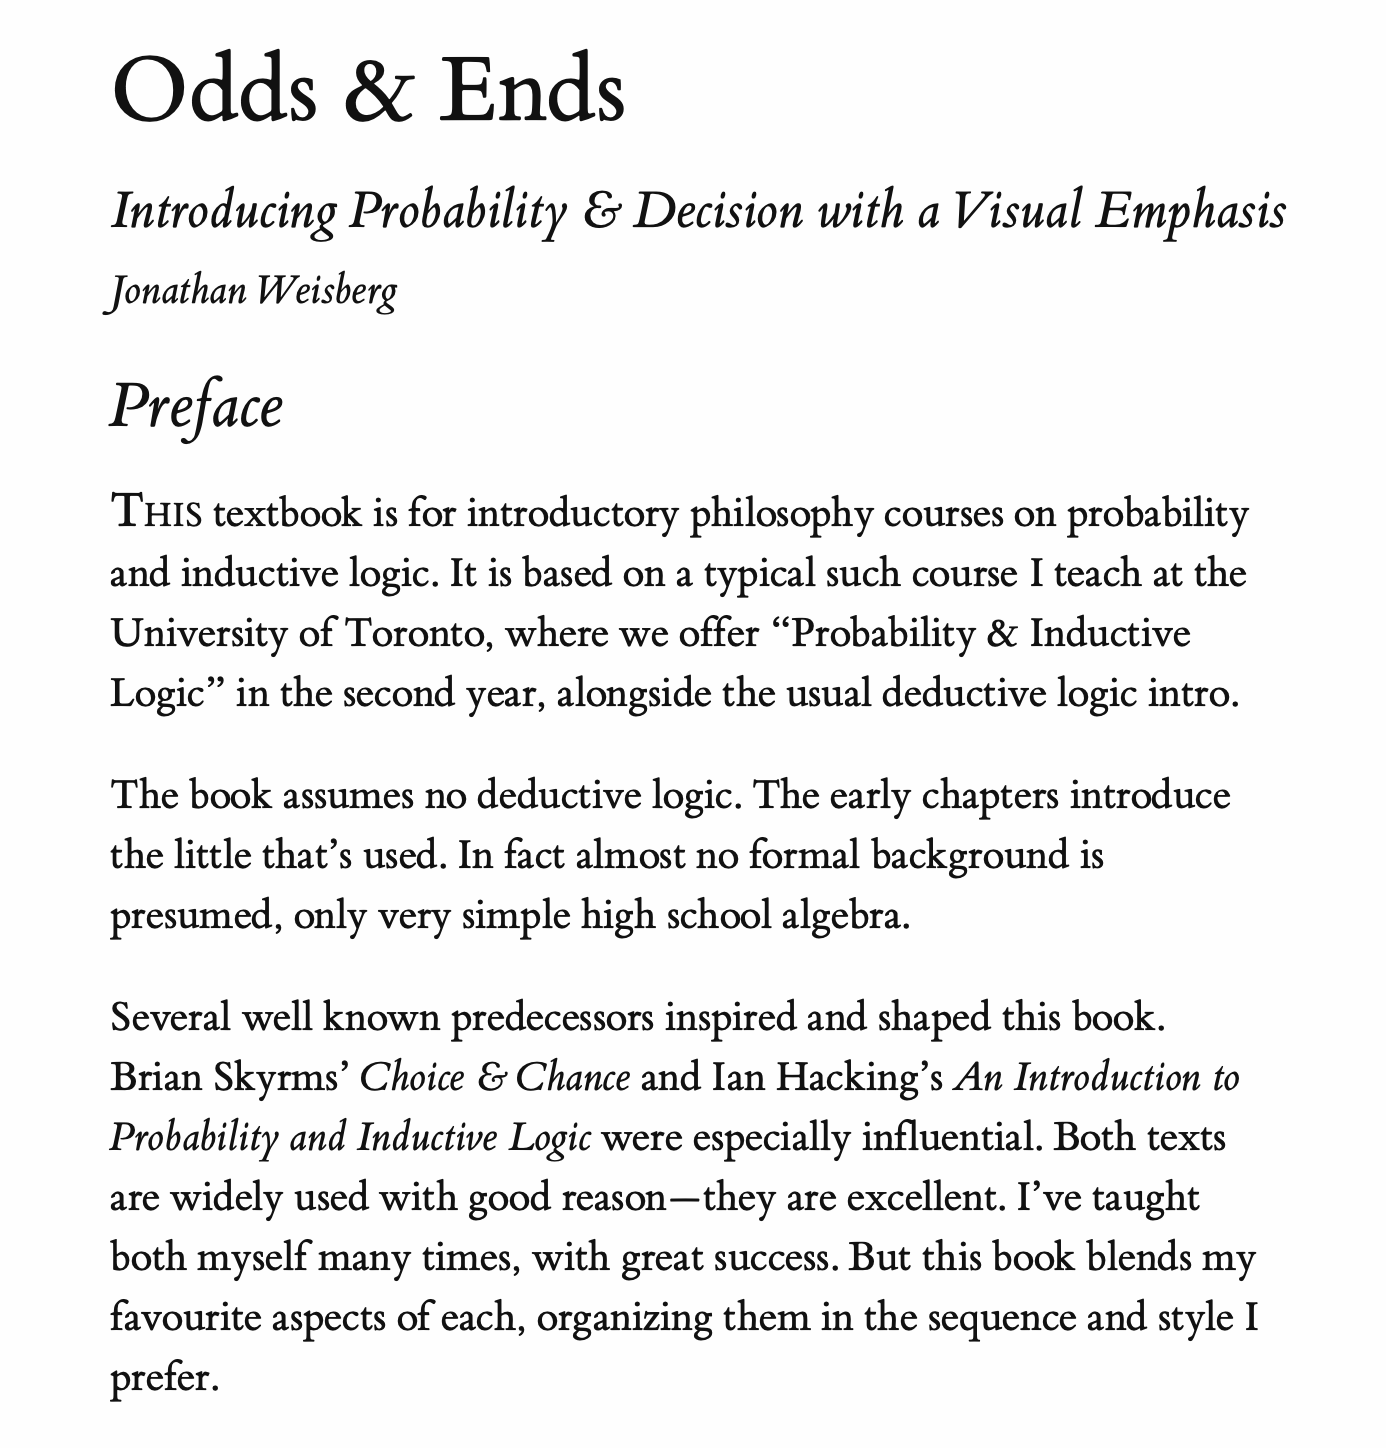
\includegraphics[width=\textwidth,height=0.8\textheight]{../images/1_1_Odds_and_Ends.png}
\caption{\url{https://jonathanweisberg.org/vip/}}
\end{figure}
\end{frame}

\begin{frame}{Boxes and Diamonds}
\protect\hypertarget{boxes-and-diamonds}{}
\begin{figure}
\centering
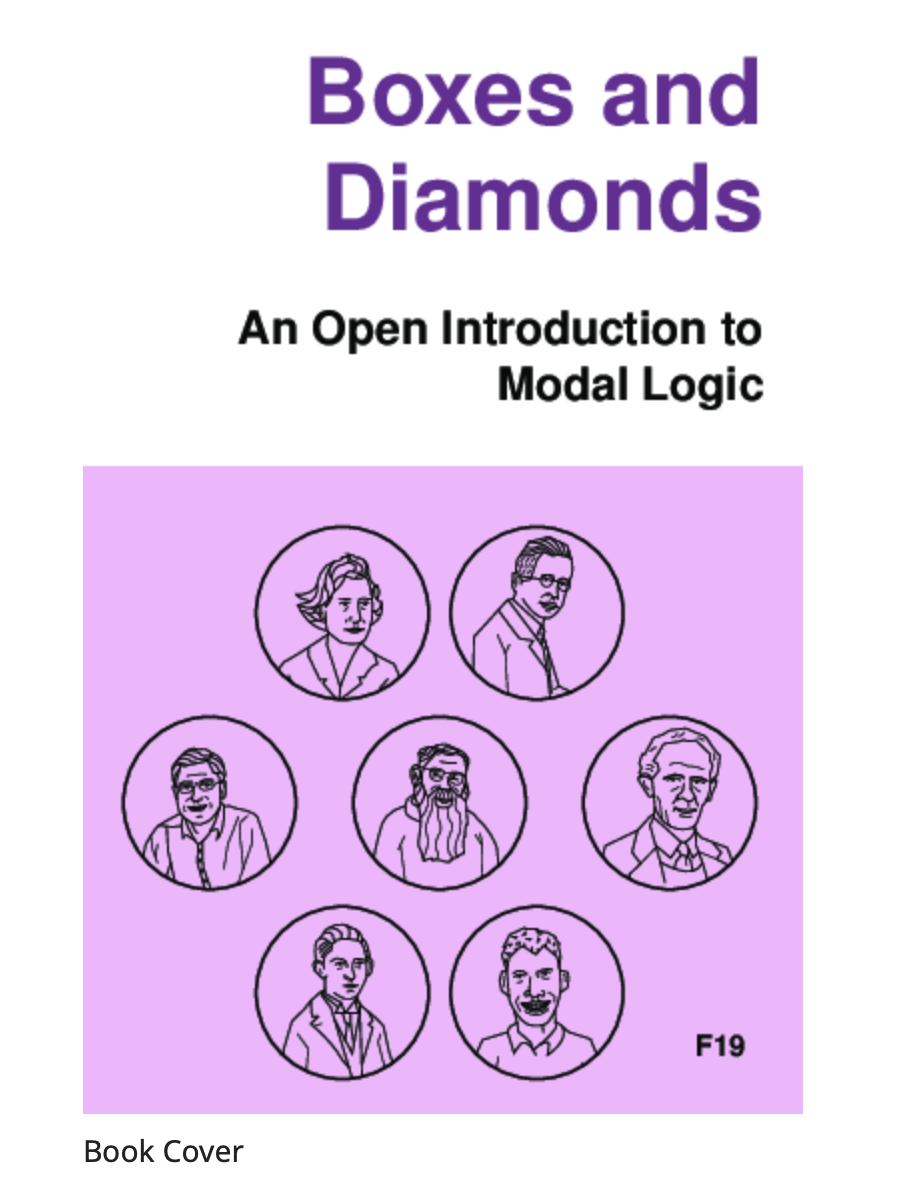
\includegraphics[width=\textwidth,height=0.8\textheight]{../images/1_1_Boxes_and_Diamonds.png}
\caption{\url{https://bd.openlogicproject.org}}
\end{figure}
\end{frame}

\begin{frame}
\begin{figure}
\centering
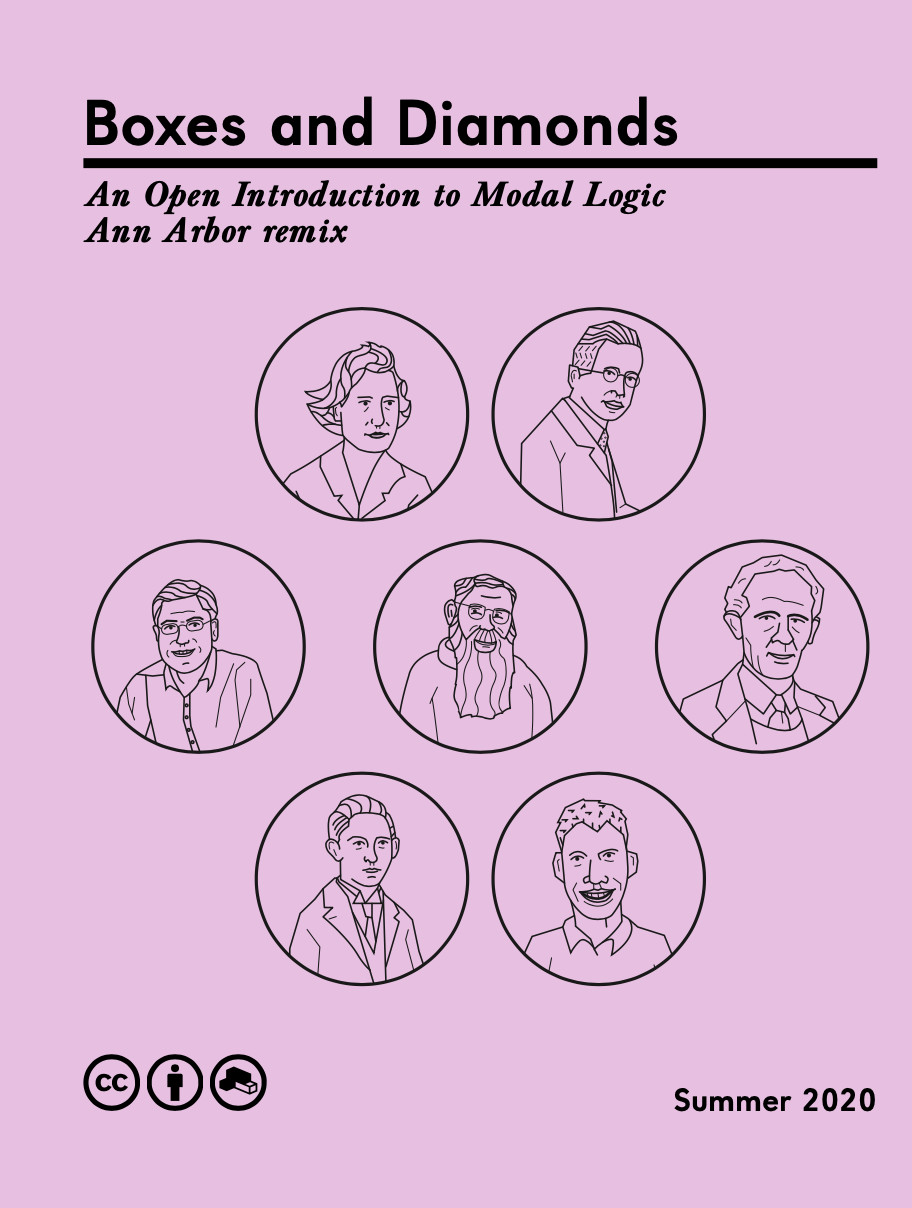
\includegraphics[width=\textwidth,height=0.8\textheight]{../images/1_1_Boxes_and_Diamonds_AA.png}
\caption{Boxes and Diamonds - Ann Arbor}
\end{figure}
\end{frame}

\begin{frame}{Logistics}
\protect\hypertarget{logistics}{}
\begin{itemize}
\tightlist
\item
  These lectures are going to be very short.
\item
  That's in part because it's really hard to retain focus through a long
  logic video, and in part because it's easier to manage uploads and
  downloads with smaller files.
\item
  So we'll typically have somewhere between 6 and 10 `lectures' each
  week, though each will be 5 to 15 minutes.
\end{itemize}
\end{frame}

\begin{frame}{Access}
\protect\hypertarget{access}{}
\begin{itemize}
\tightlist
\item
  The slides will be captioned.
\item
  The captions are produced automatically and they aren't always
  perfect.
\item
  So if they can't be used.
\item
  Access is important, and it's harder to get right for a course like
  this than for other philosophy courses, so you should hold me to a
  higher standard.
\end{itemize}
\end{frame}

\begin{frame}{Assessment}
\protect\hypertarget{assessment}{}
\begin{itemize}
\tightlist
\item
  The primary assessment will be weekly assignments, most of which will
  be administered through Canvas.
\item
  Some of them, especially in the early weeks, will be on Carnap.
\item
  These are already all posted, and they will be due each week on Friday
  at 5pm.
\item
  There are exceptions for this week, the week of the mid-term break,
  and the last week of term.
\item
  There will also be an end of term exam, also through Canvas.
\end{itemize}
\end{frame}

\begin{frame}{Syllabus}
\protect\hypertarget{syllabus}{}
\begin{itemize}
\tightlist
\item
  The syllabus is available on Canvas. Indeed, it is the first thing
  that comes up when you load Canvas.
\item
  Read it closely!!
\item
  It will tell you what we're covering each week, and where you should
  be at over time.
\end{itemize}
\end{frame}

\begin{frame}{For Next Time}
\protect\hypertarget{for-next-time}{}
We'll start on saying what arguments are, in the special sense we're
interested in.
\end{frame}

\end{document}
